\documentclass{article}

\usepackage[pdftex]{graphicx}
\usepackage[czech]{babel}
\usepackage[utf8]{inputenc}
\usepackage{enumitem}
\usepackage{amsmath}
\usepackage{url}
\usepackage{listings}
\usepackage{caption}
\usepackage[usenames,dvipsnames,svgnames,table]{xcolor}

\usepackage[pdftex]{hyperref}
\hypersetup{colorlinks=true,
  unicode=true,
  linkcolor=black,
  citecolor=black,
  urlcolor=black,
  bookmarksopen=true}

\usepackage{xcolor}
\colorlet{mygray}{black!30}
\colorlet{mygreen}{green!60!blue}
\colorlet{mymauve}{red!60!blue}
\lstset{
	backgroundcolor=\color{gray!10},  
	basicstyle=\ttfamily,
	columns=fullflexible,
	breakatwhitespace=false,      
	breaklines=true,                
	captionpos=b,                    
	commentstyle=\color{mygreen}, 
	extendedchars=true,              
	frame=single,                   
	keepspaces=true,             
	keywordstyle=\color{blue},      
	language=c++,                 
	numbers=none,                
	numbersep=5pt,                   
	numberstyle=\tiny\color{blue}, 
	rulecolor=\color{mygray},        
	showspaces=false,               
	showtabs=false,                 
	stepnumber=5,                  
	stringstyle=\color{mymauve},    
	tabsize=3,                      
	title=\lstname                
}

\usepackage[numbers,sort&compress]{natbib}

\newcommand*\justify{
  \fontdimen2\font=0.4em
  \fontdimen3\font=0.2em
  \fontdimen4\font=0.1em
  \fontdimen7\font=0.1em
  \hyphenchar\font=`\-
}

\author{Martin Úbl}

\title{KIV/OS - cvičení č. 5}

\begin{document}

\maketitle



\section{Obsah cvičení}

\begin{itemize}
	\item alokátor paměti
	\item kernelová halda
	\item správa procesů (tasků)
	\item preemptivní round-robin plánovač
\end{itemize}

\section{Alokátor paměti}

Alokace paměti je obecně poměrně složitý problém, pokud to chceme udělat správně a co nejefektivněji. My implementujeme v rámci cvičení takový alokátor, který bude pouze velmi primitivní. Rozhraní však bude mít finální a lepší implementace pak bude ponechána na další cvičení.

Nyní náš operační systém nezná např. ani stránkování -- to přibyde až v některém z dalších cvičení. Alokátor proto moc optimalizovat nebudeme, jelikož schéma alokace pak bude určitě odlišné. Mohli bychom ale už trochu počítat s tím, že budeme chtít alokovat stránky o nějaké konkrétní velikosti. Rovněž rovnou počítejme s tím, že oblast, ve které chceme alokovat, bude nějak zdola a shora omezena.

Definujme si proto soubor \texttt{memmap.h}, kde si tyto meze stanovíme. Oblast začátku můžeme zvolit v podstatě libovolně tak, aby se nepřekrývala s kódem (a daty) jádra. Pro teď si zvolme nějaký počátek ručně, v budoucnu však můžeme například použít již známý trik -- v linker skriptu definovat zarážku za poslední sekcí a tu si vyzvednout. Pak je třeba ji zarovnat na nejbližší vyšší násobek velikosti stránky a lze ji použít.

Horní mez stanovme dle možností architektury a desky. V manuálu se dočteme, že nejbližší horní hranicí je memory-mapped IO region. Pak můžeme horní mez nastavit prostě na \texttt{Peripheral\_Base}. Pozor ale -- naše zařízení zdaleka tolik fyzické paměti nemá. Řešením by mohlo být například vyzvednutí skutečného rozsahu paměti pomocí mailbox mechanismu. To ale není obsahem tohoto cvičení.
\newpage
Obsah souboru \texttt{memmap.h} pak může vypadat třeba takto:
\begin{lstlisting}
namespace mem
{
  constexpr uint32_t LowMemory = 0x20000;
  constexpr uint32_t HighMemory = Peripheral_Base;
  constexpr uint32_t PageSize = 0x4000;
  constexpr uint32_t PagingMemorySize =
                           HighMemory - LowMemory;
  constexpr uint32_t PageCount =
                      PagingMemorySize / PageSize;
}
\end{lstlisting}

Pokud to ještě v tento moment není zřejmé, operujeme v módu, kdy je každý kus paměti přímo přístupný a jeho adresa není nijak překládána. Pokud se tedy jádro v jakýkoliv moment rozhodne, že chce něco zapsat do paměti na adrese \texttt{0x00123456}, tak se to prostě s největší pravděpodobností povede.

Implementací alokátoru vlastně všechnu dostupnou paměť \uv{přidělíme} právě jádru, a alokátor bude tuto paměť spravovat. Měl by podporovat jak alokaci, tak i dealokaci bloku paměti. Z podstaty věci ale samotný alokátor neví, komu paměť přiděluje -- to pak je otázkou příslušného \uv{správce}. Tím je třeba správce haldy jádra, správce procesů a tak dále. Tento správce zodpovídá jak za \uv{úměrnou} alokaci, tak za správnou a úplnou dealokaci. Rovněž může dále vnitřně paměť rozdělovat na menší kousky -- to typicky budeme chtít jak u haldy jádra, tak i u procesů. K tomu ale zase později.

Jednou z nejjednodušších implementací alokátorů stránek (resp. později rámců) je bitová mapa. V té každý bit reprezentuje jednu stránku (rámec) paměti, přičemž hodnota \uv{vypnuto} znamená, že je blok volný a \uv{zapnuto}, že byl někomu přidělen. Jelikož víme, kolik stránek můžeme maximálně alokovat (\texttt{PageCount}), tak také víme, jak velkou bitovou mapu budeme potřebovat.

Uveďme příklad. Za předpokladu, že je paměť velká 512 MiB ($512*1024*1024$ B) a stránka (rámec) má velikost \texttt{0x4000} (16 kiB, $16*1024$ B), pak tato bitová mapa musí čítat 32768 bitů (4096 B, tedy 4 kiB). Tento výpočet lze provést v čase překladu přímo z konstant. Obětování 4 kiB z paměti pro bitmapu, která reprezentuje 512 MiB paměťový prostor není zase tolik. Jde to ale samozřejmě trochu lépe a efektivněji -- o tom více pojednávají přednášky KIV/OS nebo KIV/ZOS. Pro jednoduchost tady na cvičení implementujme bitovou mapu s algoritmem typu \emph{first-fit}, tedy $O(n)$ alokátorem, který hledá první volný blok od začátku alokovatelné paměti.

Mějme tedy třídu \texttt{CPage\_Manager}, která bude naším alokátorem. Ta bude obsahovat metodu \texttt{Alloc\_Page()}, která bude alokovat novou stránku a bude vracet adresu prvního bajtu (nebo 0, pokud žádná stránka není volná). Dále bude obsahovat metodu \texttt{Free\_Page(uint32\_t addr)}, která bude přejímat adresu prvního bajtu stránky k uvolnění jako parametr a stránku bude ve své implementaci uvolňovat.

Implementujeme bitmapový \emph{first-fit}, a tedy potřebujeme mít alokovanou bitmapu. Ve třídě proto vytvořme atribut, který bude představovat bitovou mapu alokovatelné paměti \texttt{uint8\_t mPage\_Bitmap[mem::PageCount / 8];}.

Samotná implementace pak musí obsahovat inicializaci (zde nejlépe asi konstruktorem), ve které označíme všechny bloky za volné:
\begin{lstlisting}
CPage_Manager::CPage_Manager()
{
  for (int i = 0; i < sizeof(mPage_Bitmap); i++)
    mPage_Bitmap[i] = 0;
}
\end{lstlisting}
Alokace pak probíhá snadno -- nalezením prvního oktetu stránek, který není celý alokovaný (abychom to trochu urychlili), v něm nalezení volné stránky a následným označením a vrácením:
\begin{lstlisting}
uint32_t CPage_Manager::Alloc_Page()
{
  uint32_t i, j;
	
  for (i = 0; i < mem::PageCount; i++)
  {
    if (mPage_Bitmap[i] != 0xFF)
    {
      for (j = 0; j < 8; j++)
      {
        if ((mPage_Bitmap[i] & (1 << j)) == 0)
        {
          const uint32_t page_idx = i*8 + j;
          mPage_Bitmap[page_idx / 8] |= 1 << (page_idx % 8);
          return mem::LowMemory + page_idx * mem::PageSize;
        }
      }
    }
  }

  return 0;
}
\end{lstlisting}
Uvolnění je pak již snadné -- stačí příslušný bit vynulovat:
\begin{lstlisting}
void CPage_Manager::Free_Page(uint32_t addr)
{
  const uint32_t page_idx = addr / mem::PageSize;
  mPage_Bitmap[page_idx / 8] &= ~(1 << (page_idx % 8));
}
\end{lstlisting}
V systémech, kde je nutné dbát na bezpečnost (typicky spíše interaktivní systémy) je možné při dealokaci ještě systémově přemazat obsah dealokované paměti (nějakým vzorem nebo náhodnými daty) -- pokud by k tomu nedošlo, ve stránce byla nějaká citlivá data (hesla, šifrovací klíče, ...) a stránku si pak alokoval nějaký jiný proces, k datům by pak měl přístup.

\section{Kernelová halda}

Nyní již máme způsob, jakým přidělovat stránky (rámce) paměti. Jádro ale potřebuje často alokovat malé kousky paměti pro relativně drobné struktury, a proto potřebujeme mít možnost stránky rozmělnit na drobnější kousky. Jinak by došlo k docela velkému plýtvání a výsledkem by bylo silně neefektivní využití paměti. Proto implementujme způsob, jakým toto dělení bloků umožnit.

Pro tento moment implementujeme pouze jednoduchý přímočarý algoritmus, který bude dodržovat rozhraní, ale zatím nebude představovat nic příliš efektivního -- to bude až obsahem úkolu za body, a kompletní řešení pak bude zpřístupněno.

Definujme tedy rozhraní (resp. abstraktní třídu) pro správce haldy:
\begin{lstlisting}
class IHeap_Manager
{
  public:
    virtual void* Alloc(uint32_t size) = 0;
    virtual void Free(void* mem) = 0;

    template<class T>
    T* Alloc()
    {
      return reinterpret_cast<T*>(Alloc(sizeof(T)));
    }
};
\end{lstlisting}

Toto rozhraní implementujeme pro teď pouze jednoduchým alokátorem, který umí alokovat inkrementálně kusy paměti, ale neumí dealokovat.

Správce haldy při požadavku o alokaci zjistí, zda má požadovanou paměť k dispozici (má ještě volno v přiděleném rámci). Pokud ne, alokuje si nový rámec paměti. Zarážku posune o požadovaný počet bajtů a původní hodnotu zarážky vrátí jako návratovou hodnotu volání funkce \texttt{Alloc()}. Zarážky nijak neukládá, pouze inkrementuje a vrací. To je pro nás momentálně dostačující. Do produkčního kódu by se pochopitelně podobný správce nejspíš nedostal -- jednak není úplně efektivní a jednak ani neumí dealokovat. Lepším algoritmem by mohl být například správce haldy, který si uchovává seznam alokovaných a volných míst ve spojovém seznamu. Více viz sekce s úkolem za body.

Implementace pak může vypadat nějak takto:
\begin{lstlisting}
class CKernel_Heap_Manager : public IHeap_Manager
{
  private:
    void* mStop = nullptr;
    uint32_t mRemaining = 0;

  public:
    CKernel_Heap_Manager();

    void* Alloc(uint32_t size) override
    {
      if (size > mem::PageSize)
        return nullptr;
      if (mRemaining < size)
      {
        mStop = sPage_Manager.Alloc_Page();
        mRemaining = mem::PageSize;
      }
  
      mRemaining -= size;
      void* old = mStop;
      mStop += size;
      return old;
    }

    void Free(void* mem) override
    {
      // :(
    }
};
\end{lstlisting}

Pochopitelně vyvstává spousty problémů, které vyplývají z takto primitivní implementace. Ty ale nechme pro teď být, vyřešíme je později. V tomto cvičení se potřebujeme věnovat něčemu jinému.

\section{Správa procesů}

Každý proces musí být reprezentován přepravkou, která konzervuje jeho stav. Běžně se takové přepravce říká Process Control Block (PCB) a my ji pro teď implementujeme opět jen v minimalistické podobě. V průběhu dalších cvičení pak budeme přidávat další obsah (např. mutexy, otevřené soubory, ...).

Stěžejní je pak ještě stav procesu -- ten si označme výčtovým typem:
\begin{lstlisting}
enum class NTask_State
{
  New,
  Runnable,
  Running,
  Blocked,
  Zombie
};
\end{lstlisting}
Tady je nutné poznamenat, že momentálně implementujeme procesy, \uv{jako kdybychom implementovali interaktivní systém}. Později (v druhé polovině předmětu) budeme implementaci procesů předělávat tak, aby odpovídala filozofii systémů reálného času a abstrakcí souhlasila s konceptem tasků. Pro teď je ale snazší se držet interaktivních systémů.

Jak jsme se dozvěděli na minulých cvičeních, procesor může pracovat v několika různých režimech. Jedním z nich je režim uživatelský, do kterého časem budeme umisťovat naše procesy -- nyní je však nechme v supervizor režimu. Teď je stěžejní umět mezi procesy přepínat tak, aby to bylo naprosto transparentní (vyjma určitého zpoždění, kterému se při sdílení času jednoho procesorového jádra nevyhneme).

Z výše uvedeného vyplývá, že mezi procesy bude třeba sdílet registry procesoru. Jelikož zásobník procesu zůstane nedotčený, můžeme na něj ukládat registry daného procesu při jeho přechodu ze stavu \emph{Running}. Při opětovném naplánování tyto registry z jeho zásobníku zpět vyzvedneme, čímž bude toto využití pro proces transparentní. Jediné registry, které budeme potřebovat skutečně ukládat někam do paměti (a PCB) jsou právě ukazatel na vrchol zásobníku a programový čítač. Přidejme nyní i link registr, který nám pomůže při prvním naplánování procesu.
\begin{lstlisting}
struct TCPU_Context
{
  unsigned long lr;
  unsigned long sp;
  unsigned long pc;
};
\end{lstlisting}
Do PCB ještě přidejme informace pro plánovač -- jakou má proces prioritu, a kolikrát již byl naplánovaný. To nám pak pomůže při přidělování časových kvant a zpětně i pro ladění. Celý PCB nyní může vypadat například takto:
\begin{lstlisting}
struct TTask_Struct
{
  TCPU_Context cpu_context;
  unsigned int pid;
  NTask_State state;
  unsigned int sched_counter;
  unsigned int sched_static_priority;
};
\end{lstlisting}

Na obrázku \ref{obr:switch} můžete vidět rámcové schéma přepínání kontextů dvou procesů. Nutno poznamenat jednu důležitou věc -- přepínání v dnešním cvičení nemá finální podobu. Pro teď se nebudeme zaobírat přepínáním kontextu v celé kráse, protože nám ještě zbývají dvě integrální věci pro zajištění izolovaného chodu -- ochrana paměti a uživatelský režim. Nyní budeme všechny procesy držet v režimu systémovém, a tedy privilegovaném.

Rámcově bude výměna kontextu včetně přerušení probíhat tak, že:

\begin{enumerate}
	\item v rutině zpracování IRQ uložíme registr \texttt{lr} (kam se vrátit po ošetření) a \texttt{spsr} (jaký režim a stav procesoru byl) na zásobník procesu
	\item uložíme (caller-saved) registry procesu na jeho zásobník
	\item zpracujeme přerušení jak jsme zvyklí, tady zavoláme obsluhu IRQ časovače
	\item obsluha IRQ časovače zavolá plánovač
	\item plánovač rozhodne, zda je na čase naplánovat jiný proces
		\begin{itemize}
			\item pokud ano, přepne kontext
			\item pokud ne, vrací se zpět z obsluhy
		\end{itemize}
\end{enumerate}

Toto schéma v podstatě počítá s tím, že přerušený proces zůstane kontextem v obsluze přerušení. Přepnutí kontextu tedy uloží stav v momentě přepínání, a při návratu zpět se jakoby dovykoná zbytek obsluhy přerušení (tedy vlastně už jen návrat). Nakonec pak zbytek obsluhy přerušení obnoví caller-saved registry a kontext procesu zůstane nedotčen. Tímto \emph{jakoby} přelstíme mechanismus přerušení, a podsuneme mu jiný zásobník, ze kterého následně obnovuje stav.

\begin{figure}[ht]
	\centering
	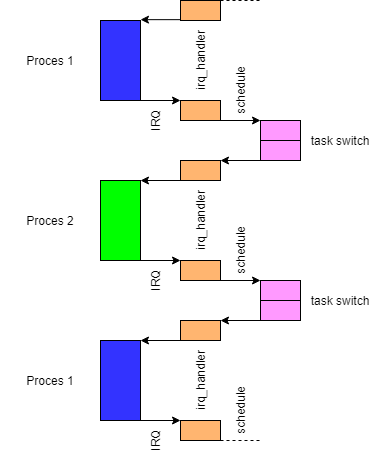
\includegraphics[width=0.6\linewidth]{OS_irq_taskswitch.png}
	\caption{Schéma přepínání kontextů pro potřeby tohoto cvičení}\label{obr:switch}
\end{figure}

Samotné přepnutí kontextu by ale jinak mohlo nahrávat řešení, že se přímo z plánovače přepneme do nového procesu (a tedy přeskočíme odrolování z IRQ handleru a kódu plánovače). To by ale znamenalo, že neuklidíme zásobník - stack pointer IRQ režimu by se nevracel zpět a netrvalo by dlouho a došlo by k podtečení zásobníku (začali bychom přemazávat data, která jsou za regionem zásobníku).

Čistě hypoteticky bychom mohli namítnout, že stačí vždy IRQ zásobník vyresetovat na začátek -- vždyť jen obsloužíme IRQ a vracíme se. To je pro teď sice pravda, jelikož okamžitě při vstupu do rutiny obsloužení IRQ zakážeme všechna přerušení a povolíme je až při přepnutí kontextu do jiného procesu, ale do budoucna to pravda už být nemusí. IRQ handler by ze své podstaty měl být reentrantní, a tedy by měl dovolovat zanořené obsluhování IRQ (jinými slovy -- obsloužit IRQ i v momentě, kdy už se nějaké obsluhuje). Pak dává naprostý smysl, že chceme zachovat zásobník v nějakém stavu, a že chceme obsluhovat přerušení tímto stylem. Teď k takové obsluze nedojde, jelikož časovač IRQ vyvolá jednou za čas, během kterého tohle jediné IRQ jsme schopni naprosto bez problému obsloužit. V budoucnu však budou IRQ vyvolávána ze spousty různých zdrojů, které nebudou tak snadno předvídatelné, jako IRQ časovače.

\subsection{Vytvoření procesu}

V tento moment předpokládejme, že si čtenář sám implementuje nějakou správu PCB (kupříkladu spojovým seznamem) a nějakou obalovou třídu, která mu dovolí s tímto seznamem řízeně manipulovat.

Nyní potřebujeme vytvořit instanci \texttt{TTask\_Struct}, která bude odpovídat novému procesu. Tu musíme naplnit informacemi tak, aby plánovač byl schopný jednak naplánovat proces poprvé (když ještě vlastně nemá žádný \uv{stav}) a v každém dalším případě.

Implementujme proto metodu pro vytvoření procesu -- měla by přejímat adresu funkce, která se má začít vykonávat (\texttt{funcptr}), vytvořit kontejner PCB, zařadit proces do fronty plánovaných procesů a vracet PID procesu:

\begin{lstlisting}
auto* task = sKernelMem.Alloc<TTask_Struct>();

task->pid = ++mLast_PID;
task->sched_static_priority = 5;
task->sched_counter = task->sched_static_priority;
task->state = NTask_State::New;

task->cpu_context.lr = funcptr;
task->cpu_context.pc =
  reinterpret_cast<unsigned long>(&process_bootstrap);

task->cpu_context.sp =
  static_cast<unsigned long>(sPage_Manager.Alloc_Page())
  + mem::PageSize;
  
PUSH_TO_PROCESS_LIST(task);

return task->pid;
\end{lstlisting}

Nyní si výše uvedené trochu rozeberme. Nejprve se naším alokátorem alokuje paměť pro PCB. Do nově vytvořené přepravky nastavíme nové PID procesu. Dále nastavíme prioritu -- pro teď půjde o hardcoded hodnotu, ale do budoucna ji chceme mít možnost volit. U plánovače typu round-robin si můžeme prioritu představit třeba jako počet časových kvant, které plánovač procesu přidělí. Následně nastavíme counter, který slouží jako ukazatel toho, kolik kvant ještě procesu zbývá. Tento čítač budeme dekrementovat pokaždé, když vyprší časové kvantum. Následně nastavíme stav procesu \texttt{New}, což indikuje, že proces ještě nebyl plánován. Je tedy technicky vzato ve stavu \texttt{Runnable}, ale abychom zbytečně nepřidávali položky do PCB, označíme si tento stav takto.

Dále vidíme, že nastavujeme registry, které se mají procesu předat při přepnutí. Technicky vzato opět potřebujeme vlastně jenom \texttt{SP} (stack pointer), ale pro názornost to ponechme takto. \texttt{LR} nastavme na funkci, kterou nastavil vnější kód k provádění v tomto procesu. Do \texttt{PC} nastavme adresu funkce \texttt{process\_bootstrap} -- ta zde bude plnit funkci jakéhosi jaderného \emph{CRT0}. Pro teď však jen přeskočí do příslušného režimu procesoru (v tomto cvičení systémový režim, do budoucna uživatelský) a provede \uv{návrat} na adresu v \texttt{LR}, a tedy vyvolá uživatelský kód.

Poté dojde k alokaci zásobníku (o velikosti jedné stránky/rámce, jelikož víc zatím neumíme) a nastavení adresy dna zásobníku do \texttt{SP} (pozn. dno je na druhé straně adresního rozsahu vzhledem k tomu, že zásobník roste do nižších adres).

Dále je v kódu obsaženo volání funkce \texttt{PUSH\_TO\_PROCESS\_LIST()}, jejíž implementace je ponechána fantazii čtenáře -- záleží, jak máte implementovaný seznam procesů a jiné podpůrné implementace.

Definujme si nyní soubor \texttt{switch.s}, který bude obstarávat nejnižší úroveň při přepínání kontextu. Implementujme v něm funkci \texttt{process\_bootstrap}:

\begin{lstlisting}
process_bootstrap:
  cps #CPSR_MODE_SYS
  add lr, pc, #8
  pop {pc}
  ;@ TODO: terminate
fin_loop:
  b fin_loop
\end{lstlisting}

Zde dojde k přepnutí do systémového režimu (v budoucnu zde budeme chtít režim uživatelský), nastavení \texttt{LR} na hodnotu \texttt{PC + 8}, což je vzhledem k délce instrukcí v ARM režimu (4 bajty) o 2 instrukce dál, tedy vlastně v nekonečné smyčce \texttt{fin\_loop}. Tady si zatím necháme stub implementace, jelikož nemáme implementovaná systémová volání. Na místě, kde nyní sedí \texttt{TODO} bude v budoucnu volání \texttt{terminate}, které odebere proces z plánovací fronty a převede ho do stavu \texttt{Zombie}.

Nyní máme první část implementovanou -- prvotní vytvoření procesu a příprava jeho běhu.

\subsection{Přepínání kontextu}

Jak již bylo nastíněno, stěžejním prvkem při přepínání kontextu bude zásobník. Na ten budeme ukládat registry (a stav) starého procesu a rovněž z něj později stav obnovovat. Celý zásobník, reprezentovaný registrem \texttt{SP}, při odplánování procesu odložíme a nahrajeme zásobník (\texttt{SP}) procesu, který je na řadě.

V případě, že proces ještě plánovaný nebyl, musíme buď stav na zásobníku vytvořit \uv{uměle}, a nebo s tím jednoduše počítat a plánovat při prvním plánování trochu jinak. Pro názornost volme druhou cestu, později se pokusíme kód (strojově) zjednodušit za cenu snížení čitelnosti.

Funkci pro přepínání kontextu budeme volat z kódu v jazyce C++. Budeme do ní potřebovat předat dva parametry -- ukazatel na kontext procesu starého (ten který \uv{odkládáme}) a procesu nového (ten který budeme plánovat). Jak již víme, volací konvence ARM předává parametry primárně prostřednictvím registrů \texttt{r0-3}, v tomto případě nám stačí dva, \texttt{r0} a \texttt{r1}.

Definujme si prototypy funkcí \texttt{context\_switch} a \texttt{context\_switch\_first} pro přepnutí kontextu opakované a první:
\begin{lstlisting}
extern "C"
{
  void context_switch(TCPU_Context* ctx_to,
                      TCPU_Context* ctx_from);
  void context_switch_first(TCPU_Context* ctx_to,
                            TCPU_Context* ctx_from);
};
\end{lstlisting}
V assembly pak implementujme jejich těla takto:
\begin{lstlisting}
context_switch_first:
  mrs r12, cpsr
  push {r14}
  push {r13}
  push {r0-r12}
  str sp, [r1, #4]

  ldr r3, [r0, #0]
  ldr r2, [r0, #8]
  ldr sp, [r0, #4]
  push {r3}
  push {r2}
  cpsie i
  pop {pc}
  
context_switch:
  mrs r12, cpsr
  push {r14}
  push {r13}
  push {r0-r12}
  str sp, [r1, #4]

  ldr sp, [r0, #4]
  pop {r0-r12}
  msr cpsr_c, r12
  pop {lr, pc}
\end{lstlisting}

Ve výše uvedeném kódu jsou první části těchto funkcí stejné (úkolem za body pak bude je přepsat tak, aby neporušovaly idiom DRY). Jde o uložení kontextu procesu tak, aby jej bylo možné později obnovit. Nejprve se uloží status registr do scratch registru, na zásobník se uloží všechny myslitelné registry a zásobník je uložen na pozici prvku \texttt{sp} přepravky, kterou jsme předali jako druhý parametr (\texttt{ctx\_to} v C++ kódu). Následně je v případě prvního přepnutí načten budoucí obsah registrů \texttt{lr}, \texttt{pc} a \texttt{sp}, stack pointer je ihned aplikován, na nový zásobník je pushnuta dvojice registrů \texttt{lr} a \texttt{pc}, jsou povolena přerušení a do registru \texttt{pc} je načtena hodnota z vrcholu zásobníku (tedy bootstrap). Jak pak vidíme v kódu bootstrap funkce, hodnota \texttt{lr} je aplikována záhy.

Pokud nejde o první přepnutí, lze vidět přesně inverzní pořadí k ukládání kontextu -- je načten nový \texttt{sp}, jsou obnoveny registry a řízení je předáno do místa návratu, tedy do adresy obsažené v původním \texttt{lr} (\texttt{r14}).

No a to je vlastně vše -- teď jen potřebujeme algoritmus plánovače, který bude umět rozlišit mezi procesy, cyklicky jim přidělovat časová kvanta a volat příslušné rutiny pro přepínání kontextu. Nesmíme zapomenout, že potřebujeme časovač, aby plánovač pravidelně spouštěl. Implementujme proto do správce procesů metodu \texttt{Schedule}, kterou bude časovač volat při obsluze svého IRQ.

Tato metoda bude pro teď vypadat nějak takto (\texttt{CProcess\_List\_Node} je přepravkou, ve které se nachází PCB a je závislá na vaší implementaci správy procesů):

\begin{lstlisting}
void CProcess_Manager::Schedule()
{
  CProcess_List_Node* current_process = Get_Current_Process();
  CProcess_List_Node* next_process = nullptr;
	
  current_process->task->sched_counter--;
  if (current_process->task->sched_counter == 0)
  {
    next_process = Select_Next_Process();
    if (next_process == current_process)
    {
      current_process->task->sched_counter =
        current_process->task->sched_static_priority; 
      return;
    }
  }

  if (next_process)
    Switch_To(next_process);
}
\end{lstlisting}

V této metodě jsme použili metody \texttt{Select\_Next\_Process()} a \texttt{Switch\_To()}. Ty budou opět tak trochu závislé na tom, jakou organizaci procesů v paměti jste zvolili a jak jste označili jednotlivé prvky pomocných struktur. Pseudokódem se však pokusme naznačit, jak by mohly vypadat.

Nejprve vybírání dalšího procesu:
\begin{lstlisting}
CProcess_List_Node* CProcess_Manager::Select_Next_Process()
{
  CProcess_List_Node* candidate = Get_Current_Process();
	
  do
  {
    candidate = GET_NEXT_PROCESS_IN_LIST();
  }
  while (candidate->task->state != NTask_State::Running &&
         candidate->task->state != NTask_State::Runnable &&
         candidate->task->state != NTask_State::New);
         
  return candidate;
}
\end{lstlisting}

Tato metoda pouze prochází seznam procesů (dle vaší implementace), dokud nenarazí na nějaký plánovatelný proces (a v případě nutnosti začne prohledávat seznam od začátku). Nutno dodat, že takto vypadá tělo pouze \uv{obyčejného} round-robin plánovače. Ten je pro systémy reálného času (a nejen pro ně) naprosto nedodstatečný a korektní variantou plánovače se budeme zaobírat v dalších cvičeních.

Metoda \texttt{Switch\_To()} může pak vypadat třeba takto:
\begin{lstlisting}
void CProcess_Manager::Switch_To(CProcess_List_Node* next)
{
  CProcess_List_Node* current_process = Get_Current_Process();
  
  TTask_Struct* old_task = current_process->task;
  TTask_Struct* new_task = next->task;
  
  if (old_task->state == NTask_State::Running)
    old_task->state = NTask_State::Runnable;
    
  bool is_first_time = (new_task->state == NTask_State::New);
  
  SET_CURRENT_TASK(next);
  new_task->sched_counter = new_task->sched_static_priority; 
  new_task->state = NTask_State::Running;
  
  if (is_first_time)
    context_switch_first(new_task, old_task);
  else
    context_switch(new_task, old_task);
}
\end{lstlisting}

Nejprve je starý proces přepnut do stavu \texttt{Runnable}, ale pouze pokud je ve stavu \texttt{Running} (pokud by byl ve stavu \texttt{Blocked}, nebylo by to žádoucí ze zjevných důvodů). Poté je rozhodnuto, zda je nový proces plánován poprvé. Interně je pak nastaven jako současný proces, je mu nastaven počet časových kvant a je přepnut do stavu \texttt{Running}. Následně je volána příslušná funkce pro přepnutí kontextu na nový proces.

\subsection{Problém - první přepnutí kontextu}

Nyní nám může ještě činit potíže úplně první přepnutí kontextu, jelikož na počátku existence plánovače žádný proces vlastně neběží. Tento problém má poměrně jednoduché řešení -- vytvoříme virtuální proces, který označuje současný kontext a donutíme plánovač, aby si myslel, že doteď nějaký proces běžel. My pak musíme volat příslušnou metodu vytvoření tohoto procesu ještě předtím, než spustíme plánovač.

Vytvořme v plánovači metodu \texttt{Create\_Main\_Process()}, která (částečně pseudokódem) může vypadat například takto:
\begin{lstlisting}
auto* task = sKernelMem.Alloc<TTask_Struct>();

task->pid = ++mLast_PID;
task->sched_static_priority = 1;
task->sched_counter = task->sched_static_priority;
task->state = NTask_State::Running;

PUSH_TO_PROCESS_LIST(task);
SET_CURRENT_TASK(next);

return task->pid;
\end{lstlisting}

Poté můžeme bez problémů spustit plánování a vše by mělo fungovat.

\subsection{Testovací procesy}

Pro otestování plánovače můžeme vytvořit dva procesy -- oba budou na UART vypisovat jednotlivé znaky, a pokud na výstupu uvidíme nějaký rozumně vyvážený mix obou znaků, plánovač nejspíš funguje správně.

\begin{lstlisting}
extern "C" void Process_1()
{
  volatile int i;
	
  sUART0.Write("Process 1\r\n");
	
  while (true)
  {
    sUART0.Write('1');
	
    for (i = 0; i < 0x10000; i++)
      ;
  }
}

extern "C" void Process_2()
{
  volatile int i;
	
  sUART0.Write("Process 2\r\n");
	
  while (true)
  {
    sUART0.Write('2');

    for (i = 0; i < 0x10000; i++)
      ;
  }
}
\end{lstlisting}

V kódu hlavní funkce pak nezapomeňme vložit kód, který vytvoří jak hlavní systémový proces, tak oba testovací:
\begin{lstlisting}
sProcessMgr.Create_Main_Process();

sProcessMgr.Create_Process(
  reinterpret_cast<unsigned long>(&Process_1));
sProcessMgr.Create_Process(
  reinterpret_cast<unsigned long>(&Process_2));
\end{lstlisting}

Po nahrání by mělo na konzoli UARTu být vidět něco v tomto duchu (pochopitelně záleží na zvolené frekvenci IRQ časovače, a tedy velikosti časového kvanta):

\begin{verbatim}
Process 1
Process 2
1212121212121212112121212211212121212121...
\end{verbatim}




\section{Úkol za body}

Vaším úkolem bude implementovat jedno z následujících dvou bodů:

\begin{enumerate}
	\item lepší kernel heap manager, který podporuje i dealokaci (např. seznam bloků a děr)
	\item generalizaci přepínání kontextu, abychom nepotřebovali dvě funkce pro context switch a stačila jen jedna
\end{enumerate}

První úkol je spíše pracný a vyžaduje trochu algoritmizace a analytického ducha. Ve své podstatě však není nijak složitý.

Druhý úkol vyžaduje práci s nízkoúrovňovým kódem a pochopení architektury. Sám o sobě vyžaduje vlastně jen malé úpravy, ale zato je třeba je velmi důkladně promyslet.

Vyberte si proto jeden z výše uvedených úkolů a implementujte, co je potřeba.

\emph{Pozn.: pokud implementujete oboje, máte stále nárok jen na jeden bod (ale navíc klidně malé bezvýznamné plus).}

\end{document}























